
\begin{figure*}[t]
  \centering
  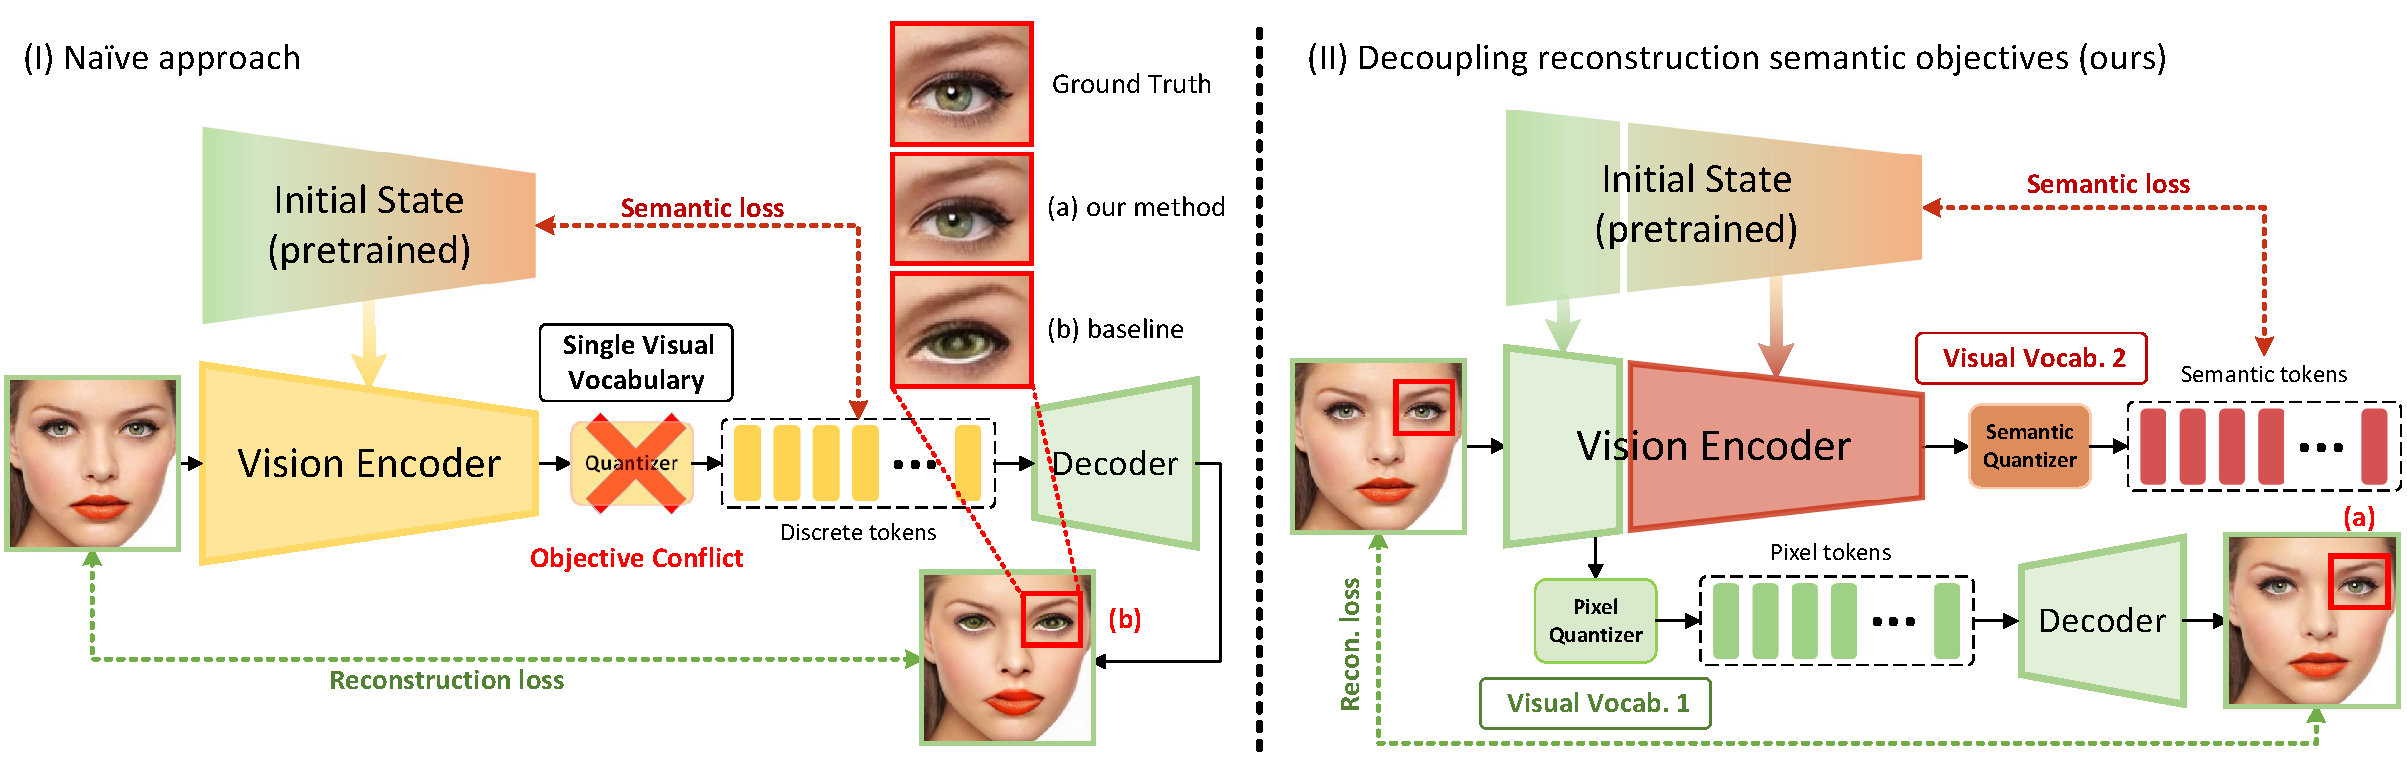
\includegraphics[width=0.92\textwidth]{imgs/tokenizer.pdf}
  % 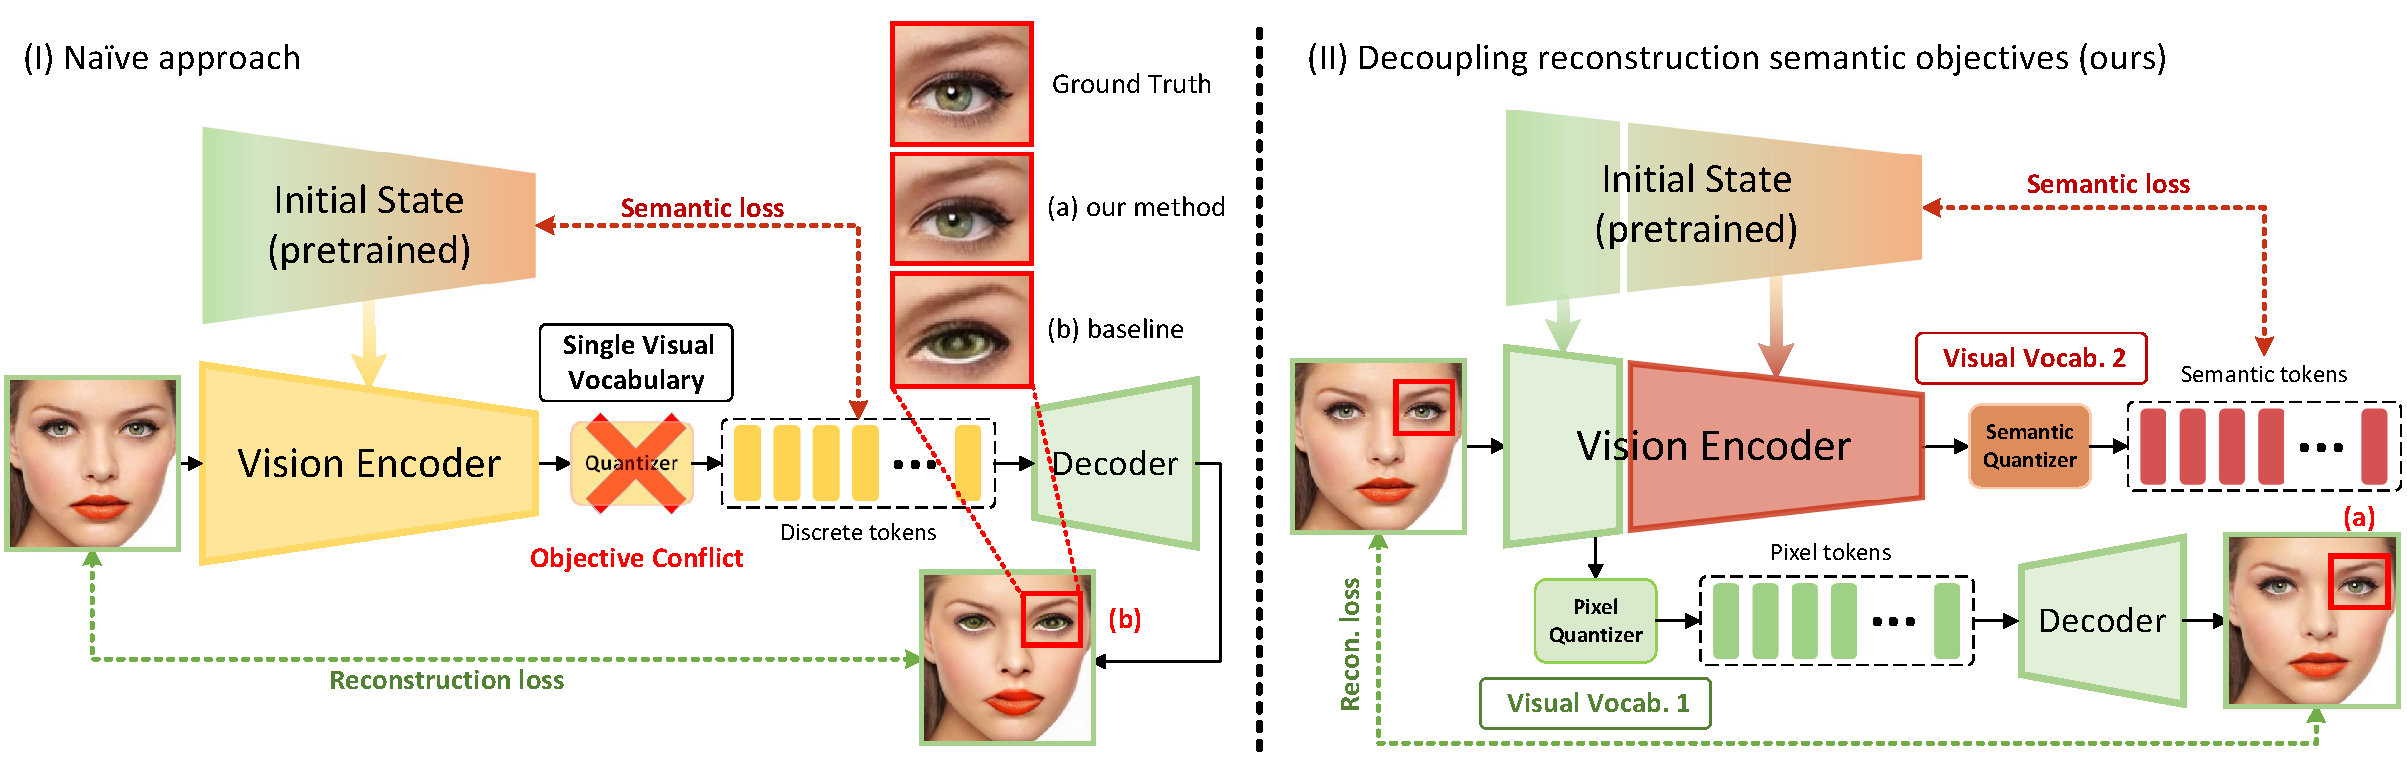
\includegraphics[width=0.475\textwidth]{imgs/tokenizer.pdf}
  \caption{
    \textbf{Comparing the design of a naive~(Left) and our decoupled approach~(Right).}
    Naively combining reconstruction and semantic loss with a single visual vocabulary leads to distorted reconstruction and degraded semantic performance. We decouple the two objectives through a hierarchy approach, where reconstruction loss is applied to supervise the shallow layers, while semantic supervision is applied to the deep layers. This enhances both reconstruction fidelity and semantic quality. Consequently, we derive two complementary visual vocabularies: a pixel codebook for low-level visual appearance, and a semantic codebook for high-level visual semantics.
    % \KY{The entire paragraph does not align with your figure. I suggest you redo this.}
  }
  \label{fig:tokenizer_framework}
  \vspace{-0.25cm}
\end{figure*}
